\chapter{Datasets}
This chapter provides an overview of the five datasets used in this Master's dissertation, all of which contain explicit ratings made by users across various item sets. Three of the datasets contain movie ratings, while the other two contain ratings of books and jokes respectively.

The MovieLens datasets are used frequently in CF research efforts. GroupLens research at the university of Minnesota is responsible for maintaining these data in four stable sets of different sizes: 100K, 1M, 10M and 20M. For the purposes of this research, the 20M was not necessary and so only the first three were used. Each set is named after the number of ratings it contains. The first two datasets use a 5 star, integer-only rating scale, while the 10M and 20M datasets each contain ratings from 0.5 - 5 stars, including half star ratings \parencite{harper2016movielens}.

The Jester dataset contains over 4.1 million ratings of 100 jokes from over 70 000 users. Ratings fall on a continuous scale between $-10.0$ and $+10.0$. The low number of items and the continuous ratings scale make this dataset notably different to the others used in this project \parencite{cf_1.2_eigentaste}.

The goodbooks-10k dataset takes its name after the fact that it contains 10 000 books, with a total of just under 6 million times by over 50 000 users \parencite{goodbooks2017}.

\section{Number of users, items and ratings}
Each dataset has a different profile in terms of the ratios between numbers of users, items and ratings. The density is calculated as the number of ratings provided as a proportion of the total number of possible user-item interactions. ML 100K -- the dataset with the fewest ratings -- has 943 unique users and 1 682 unique movie titles. This would allow a total of 1 586 126 possible user-movie ratings. Since there are only 100 000 ratings in this dataset, its density is thus $\dfrac{100000}{1.586126} = 6.30\%$. Table \ref{tab:data-summary} provides a summary of these datasets. 

\begin{table}[H]
\centering
\begin{tabular}{c | c | c | c | c | c}
\toprule
\textbf{Name} & \textbf{Rating Scale} & \textbf{Users} & \textbf{Items} & \textbf{Ratings} & \textbf{Density} \\
\midrule
ML 100K & 1--5, stars & 943 & 1 682 & 100 000 & 6.30\% \\
ML 1M & 1--5, stars & 6 040 & 3 706 & 1 000 209 & 4.47\% \\
ML 10M & 0.5--5, half-stars & 69 878 & 10 681 & 10 000 054 & 1.34\% \\
Goodbooks-10k & 1--5, stars & 53 424 & 10 000 & 5 976 479 & 1.12\% \\
Jester & -10.0--10.0, decimal & 73 418 & 100 & 4 136 210 & 56.34\% \\
\bottomrule
\end{tabular}
\caption[Data summary]{Summary of the datasets used in this project}
\label{tab:data-summary}
\end{table}

The Jester dataset has the highest density by a significant margin (56.34\%). ML 100K, 1M and the goodbooks-10k sets all use an integer rating scale between 1 and 5 stars. The ML 10M set also uses a 5 star scale, but allows half star ratings, whereas the Jester dataset uses a continuous ratings scale between -10 and +10.

In terms of size, ML 100K is the smallest with 100 thousand ratings, while the other sets all range between 1 and 10 million ratings. The Jester data set contains the most users, while ML 10M contains the most items, albeit only by a slight margin over goodbooks-10k.

\section{Distribution of ratings}
Table \ref{tab:ratings-distribution} provides a summary of the distribution of ratings across users and items in each of the datasets.

All three MovieLens datasets have a minimum of 20 ratings per user, while some of the movies have only 1 rating.

The Jester dataset has the fewest average ratings per user; however, each item is rated over 41-thousand times on average, with even the least frequently rated item having over 18-thousand ratings.

The Goodbooks-10k dataset is similar to the MovieLens datasets in terms of its distribution across items; however, every book has at least 8 ratings as opposed to the 1 rating minimum of the MovieLens sets.

\begin{table}[H]
\centering
\begin{tabular}{c | c | c | c | c | c | c}
\toprule
\textbf{Name} & \textbf{Min User} & \textbf{Max User} & \textbf{Avg User} & \textbf{Min Item} & \textbf{Max Item} & \textbf{Avg Item} \\
\midrule
ML 100K & 20 & 737 & 106 & 1 & 583 & 60 \\
ML 1M & 20 & 2 314 & 166 & 1 & 3 428 & 270 \\
ML 10M & 20 & 7 359 & 143 & 1 & 34 864 & 937 \\
Goodbooks-10k & 19 & 200 & 112 & 8 & 22 806 & 598 \\
Jester & 15 & 100 & 56 & 18 505 & 73 410 & 41 362 \\
\bottomrule
\end{tabular}
\caption[Ratings distribution]{Summary of the distribution of ratings in each dataset}
\label{tab:ratings-distribution}
\end{table}

\subsection{Number of ratings per user}
All three MovieLens datasets have a similar right-tailed distribution of the number of ratings made per user. The majority of users have made a small number of ratings -- between 1 and 100 -- with a small number of users having rated a very high number of movies.

The Goodbooks-10k dataset user ratings follow a Gaussian distribution, with the majority of users having rated between 75 and 130 books. No user has rated fewer than 19, or more than 200, books.

The Jester dataset has a fairly uniform distribution that is skewed to the right, with two distinct groups of users who have rated between 75 and 80 and between 95 and 100 respectively.

The histograms in figures \ref{fig:ML10M-users}, \ref{fig:goodbooks-users} and \ref{fig:jester-users} show the distributions of the number of ratings made per user in ML 10M, Goodbooks-10k and Jester. MovieLens 1M and 100k have similar shapes, albeit each with fewer users than the ML 10M shown in figure \ref{fig:ML10M-users}.

\begin{figure}[H]
\centering
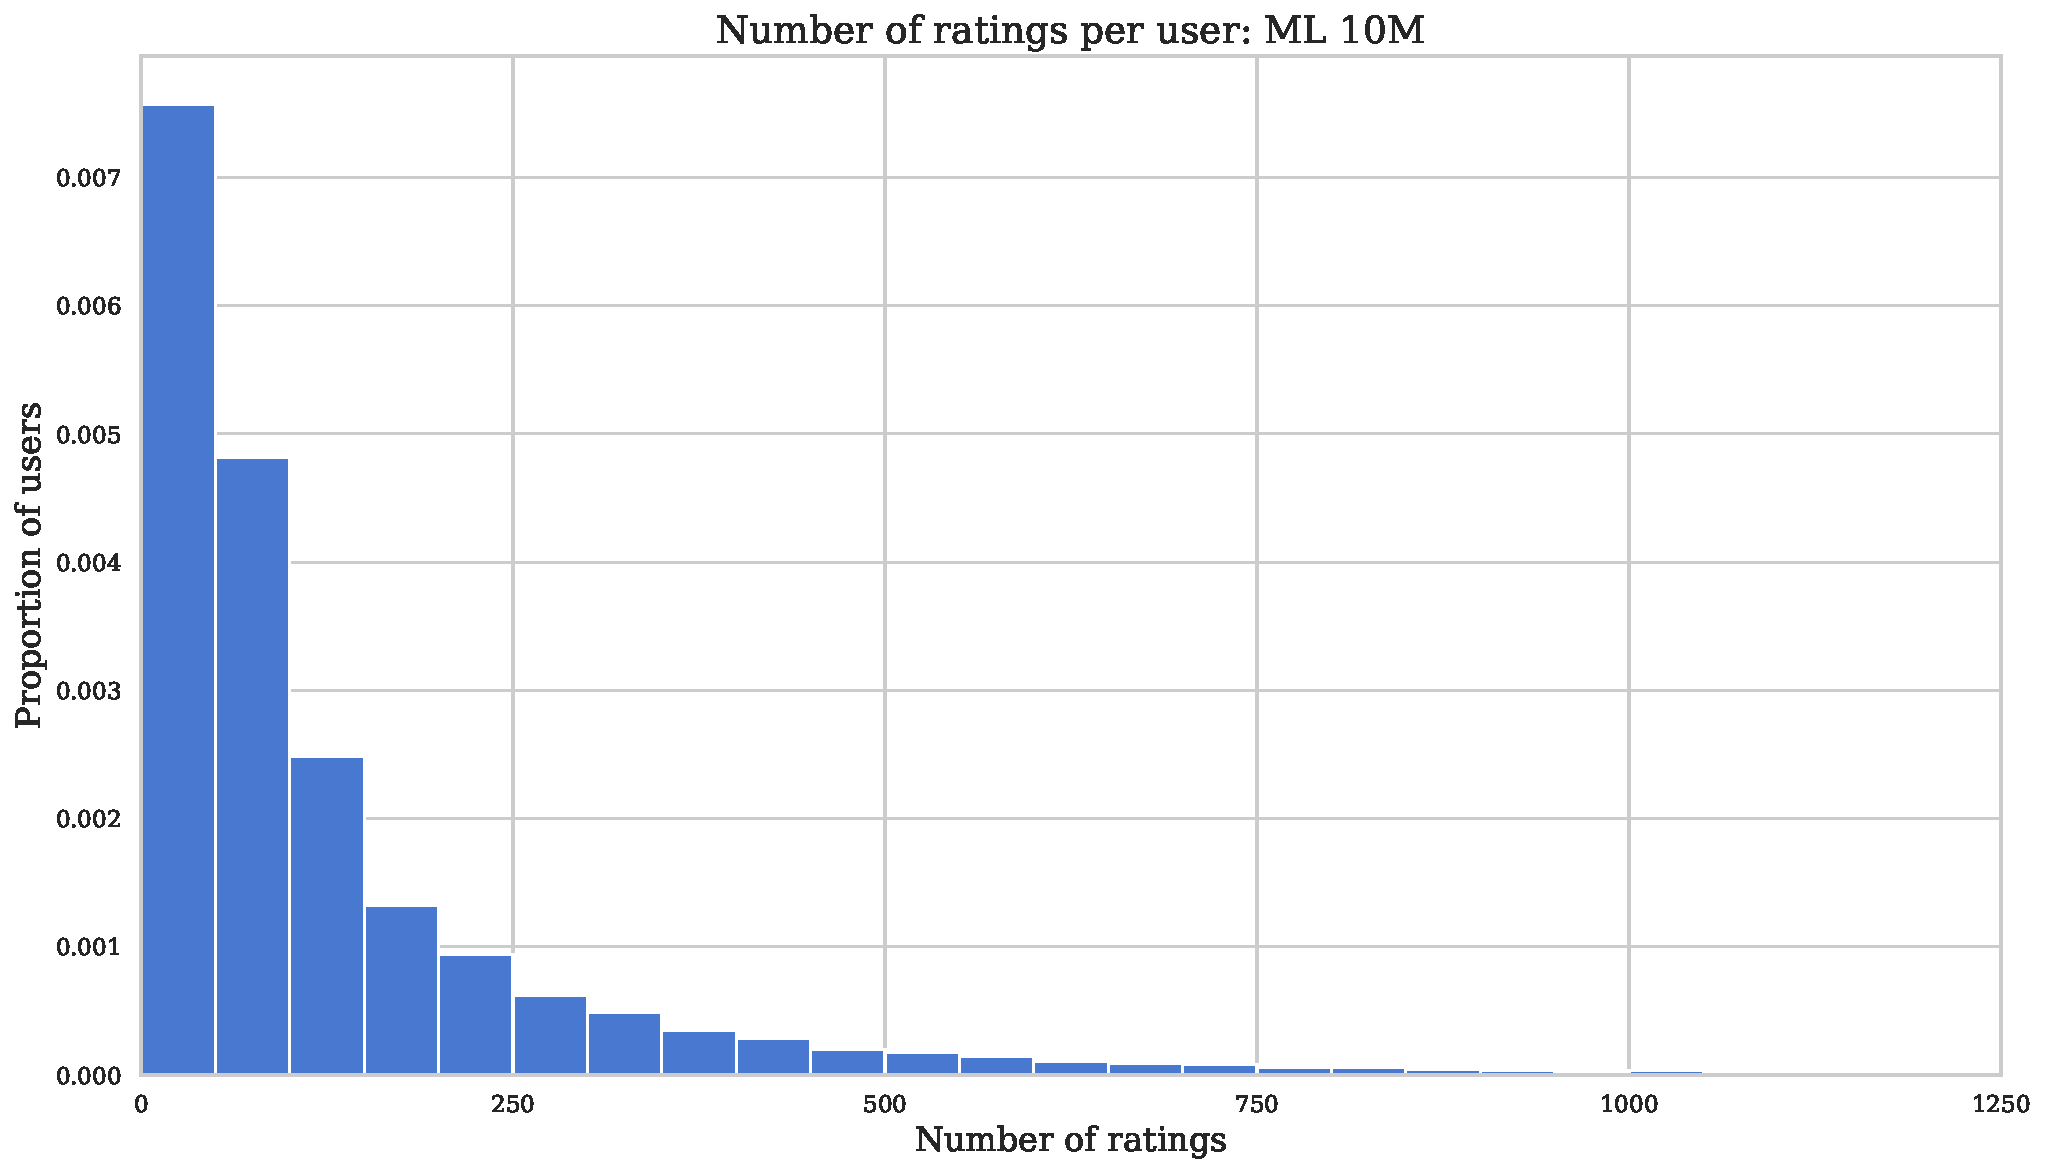
\includegraphics[width=0.75\textwidth]{Figures/3_ratings-distributions/ml_10m_user-ratings.pdf}
\caption{ML 10M number of ratings per user. Most users have rated a small number of movies.}
\label{fig:ML10M-users}
\end{figure}

\begin{figure}[H]
\centering
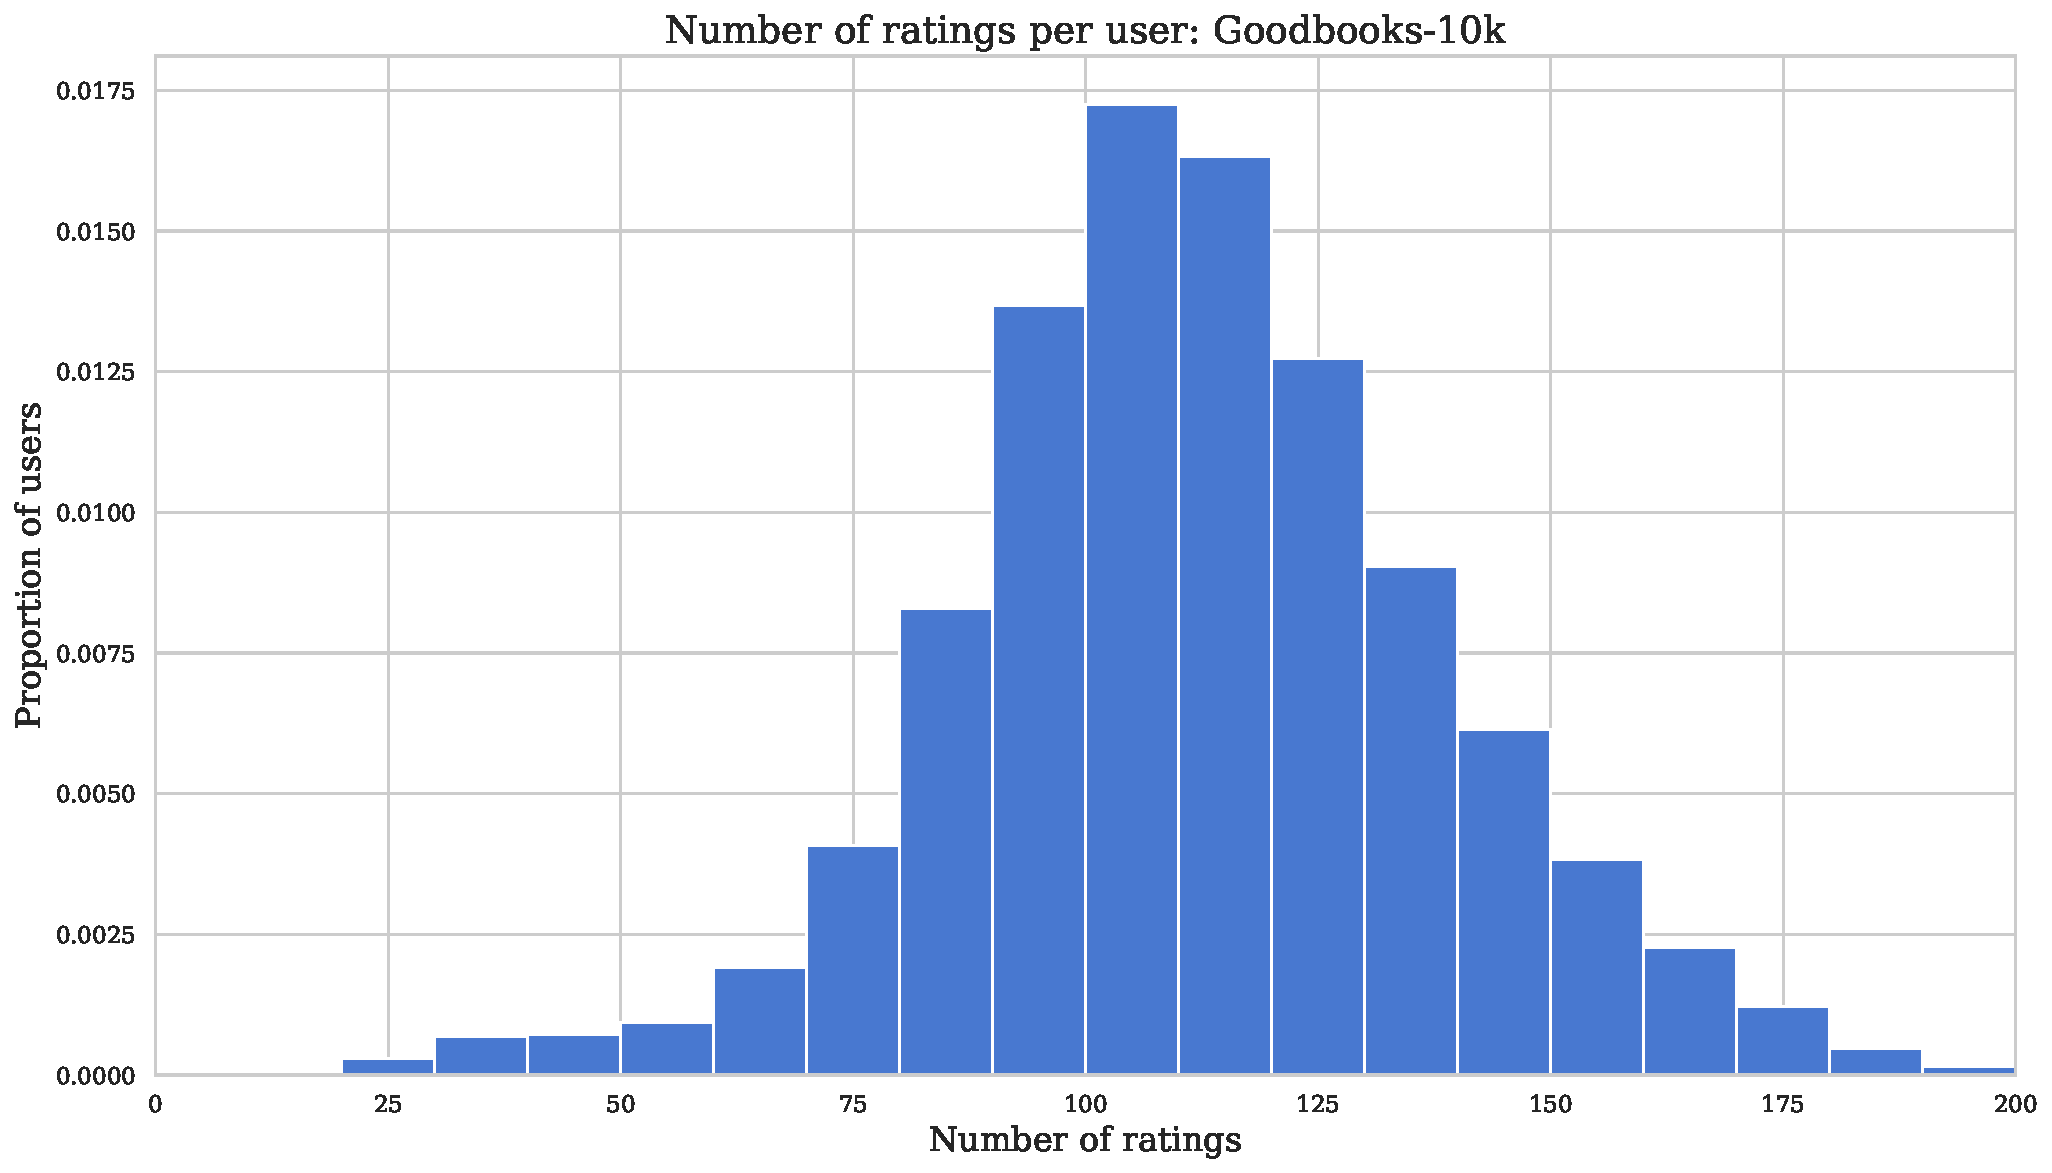
\includegraphics[width=0.75\textwidth]{Figures/3_ratings-distributions/goodbooks_user-ratings.pdf}
\caption{Goodbooks-10k number of ratings per user. Number of ratings per user is approximately normally distributed.}
\label{fig:goodbooks-users}
\end{figure}

\begin{figure}[H]
\centering
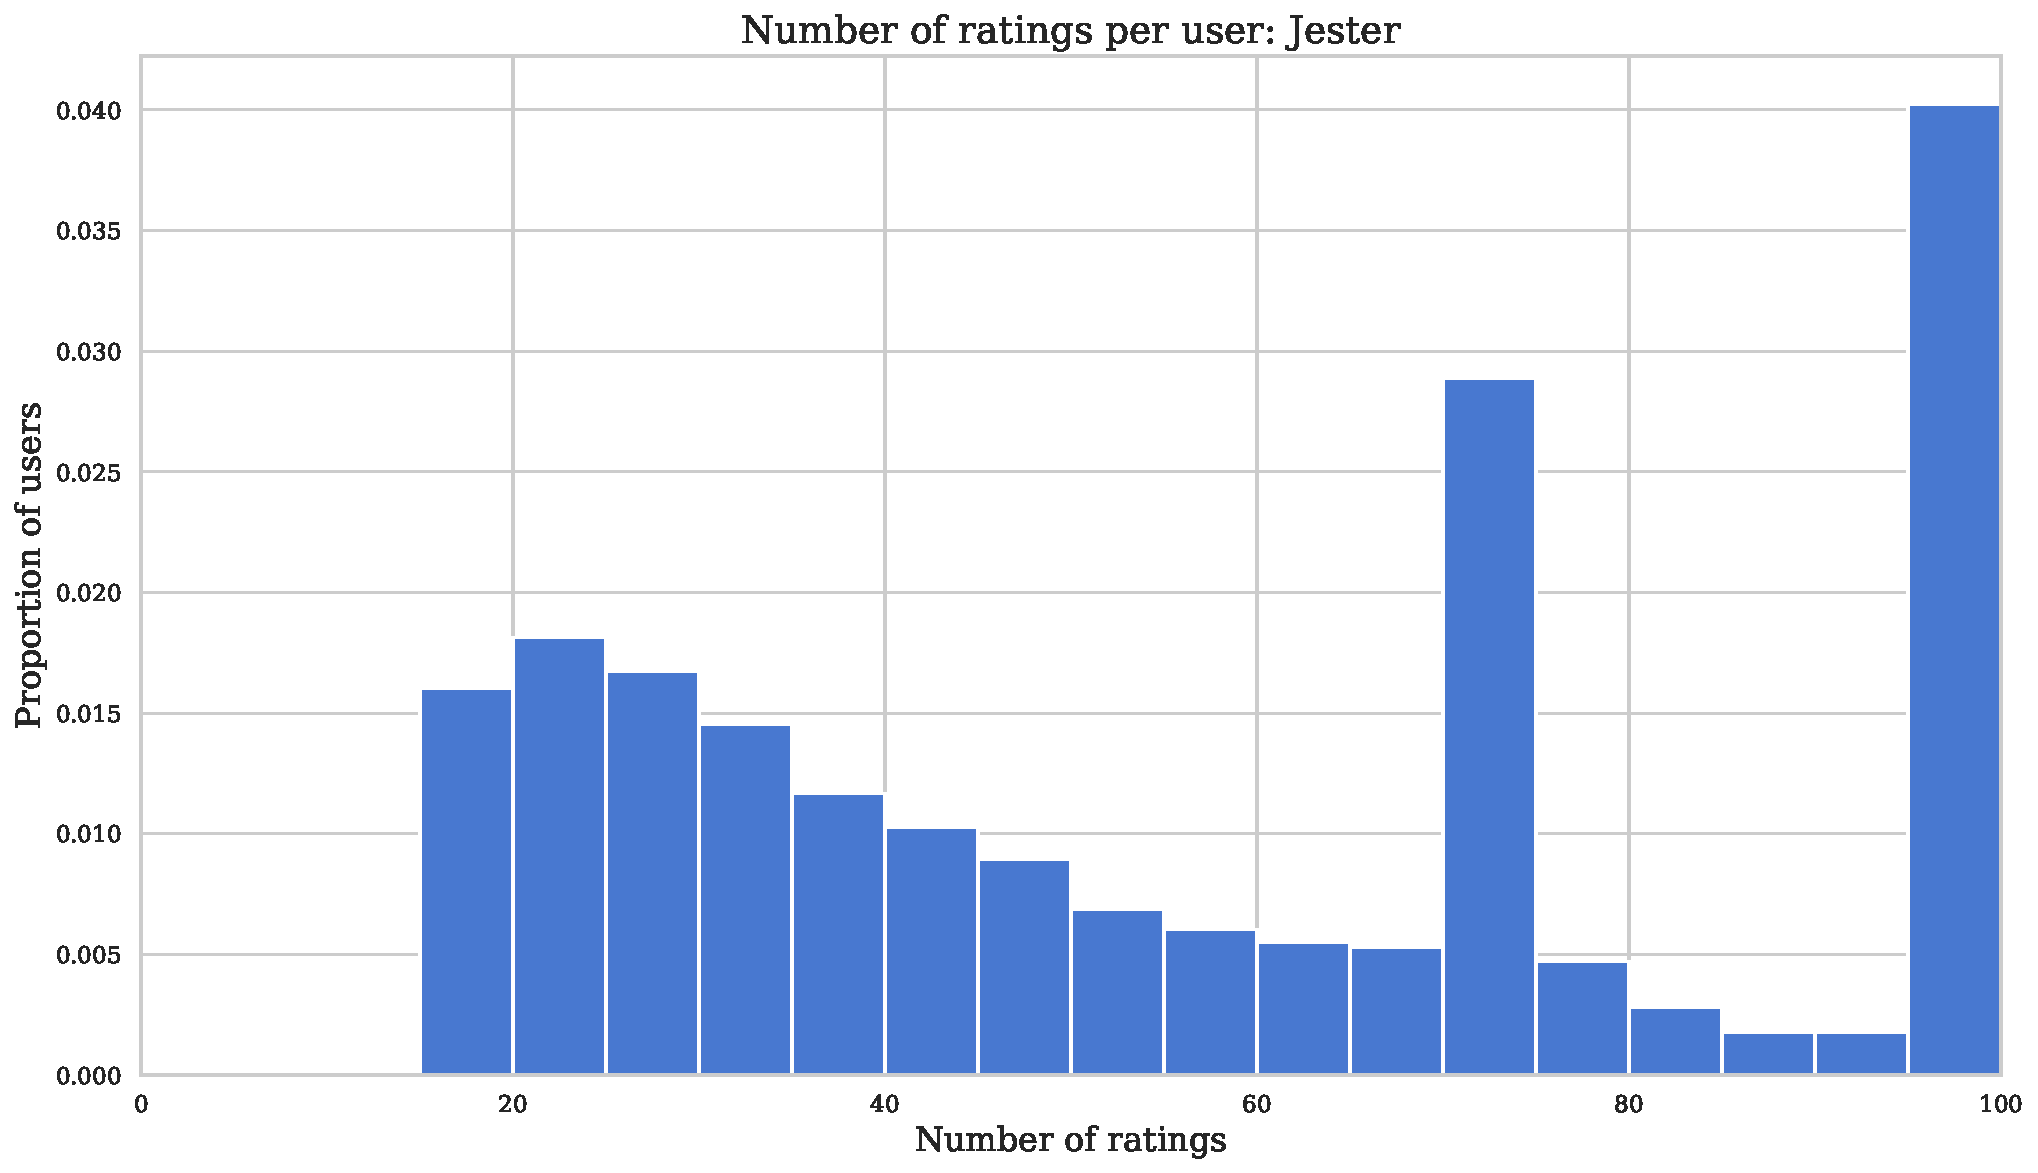
\includegraphics[width=0.75\textwidth]{Figures/3_ratings-distributions/jester_user-ratings.pdf}
\caption{Jester number of ratings per user.}
\label{fig:jester-users}
\end{figure}

\subsection{Number of ratings per item}
The number of ratings per movie in the MovieLens datasets follow a similar right-tailed distribution to the number of ratings per user; however, since there are fewer movies than users, the average number of ratings per movie is higher.

The number of ratings per book in the Goodbooks-10k dataset does not follow a normal distribution, as is the case with ratings per user. Instead, the number of ratings per book in this dataset follows a similar right-tailed pattern to the MovieLens datasets.

Since there are only 100 jokes in the Jester dataset, each joke receives a far greater number of ratings on average than the items in the other datasets. Each joke has been rated a minimum of 18 505 times, while the most ratings received by one joke is 73 410.

Figures \ref{fig:ML10M-items}, \ref{fig:goodbooks-items} and \ref{fig:jester-items} show the distributions of the number of ratings per item in each of the ML 10M, Goodbooks-10k and Jester datasets. As is the case with the distributions of the number of ratings per user, the three MovieLens datasets all have similar distributions across number of ratings per item and so only the largest of the datasets is shown below.

\begin{figure}[H]
\centering
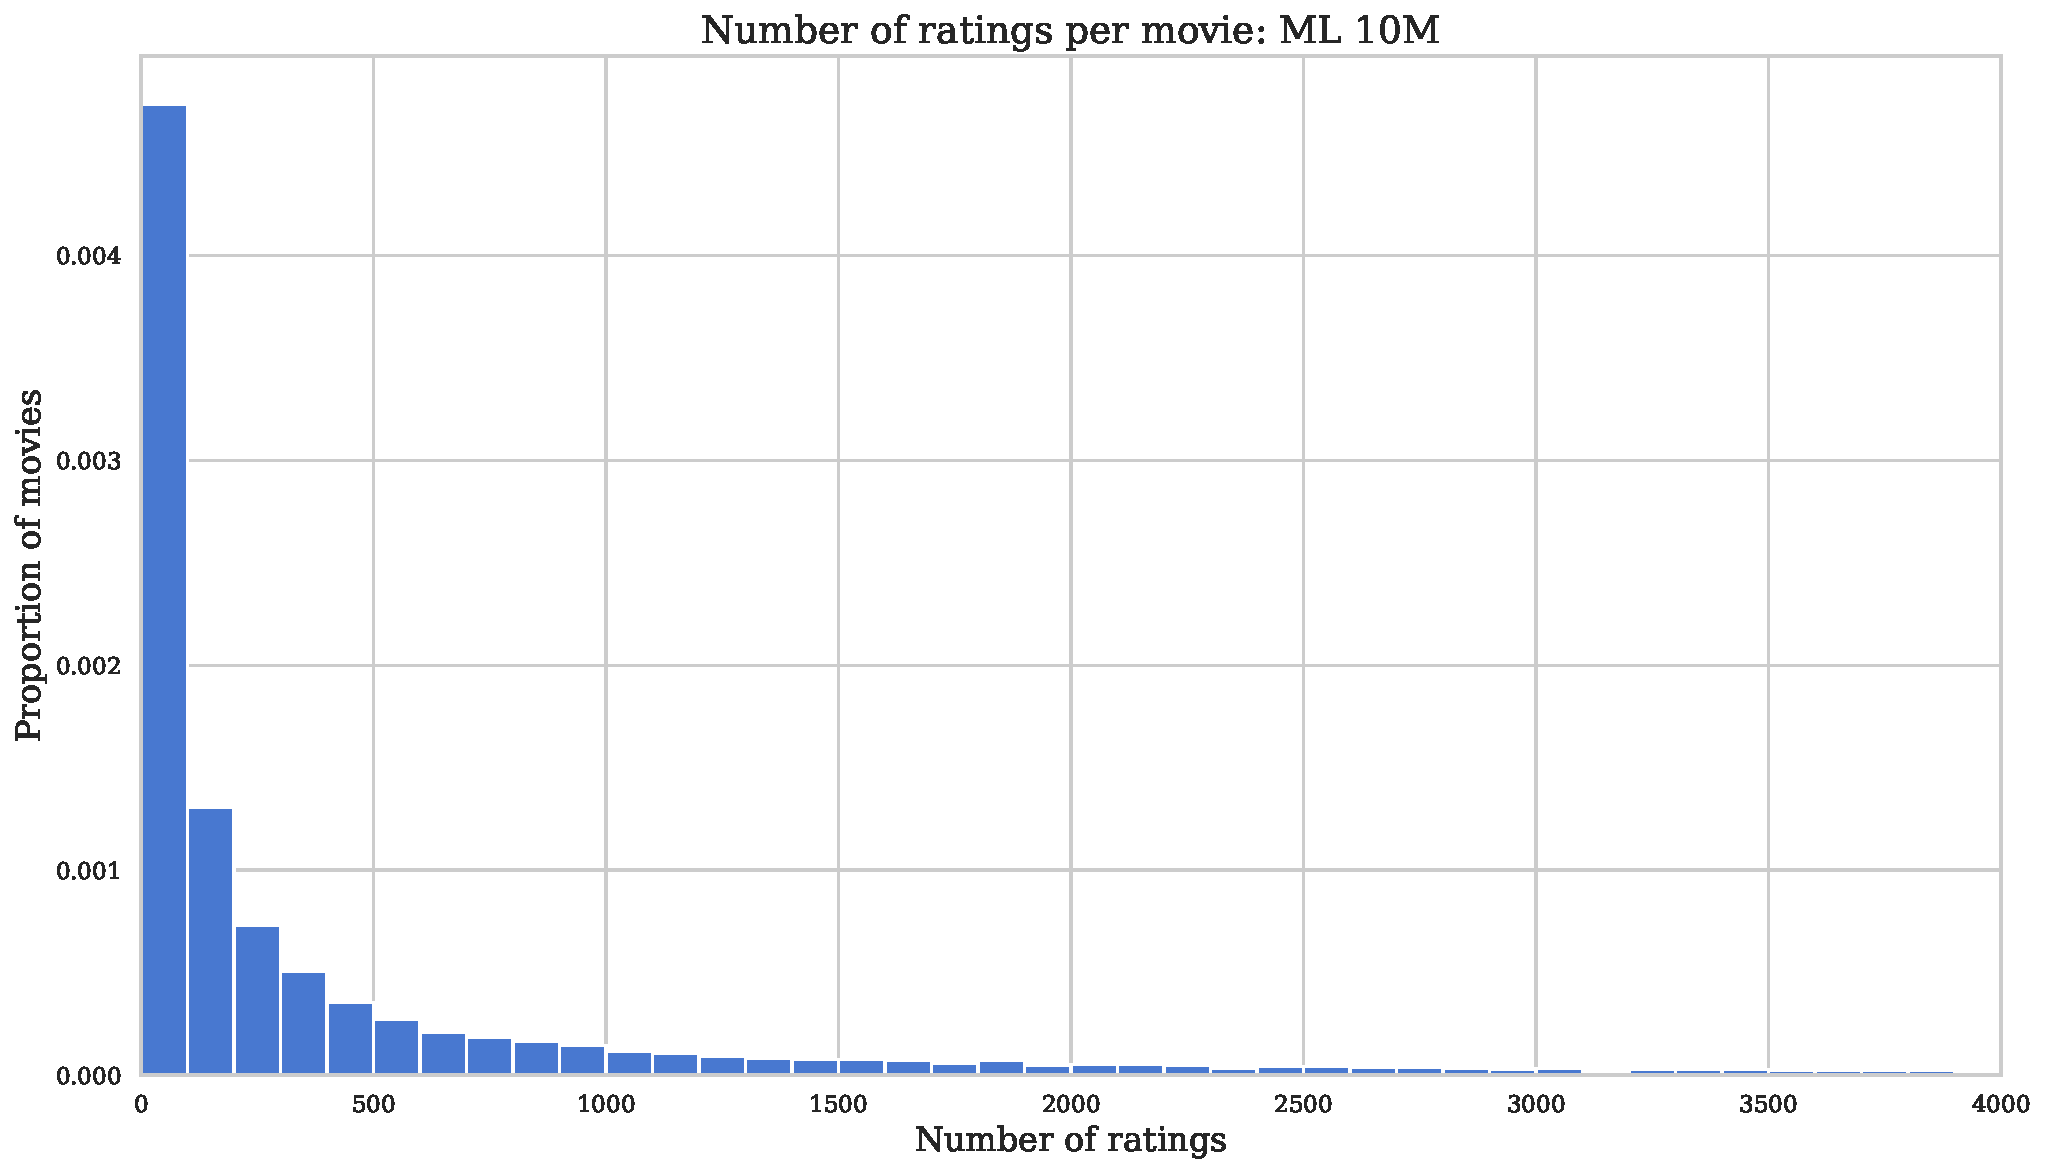
\includegraphics[width=0.75\textwidth]{Figures/3_ratings-distributions/ml_10m_movie-ratings.pdf}
\caption{ML 10M number of ratings per movie.}
\label{fig:ML10M-items}
\end{figure}

\begin{figure}[H]
\centering
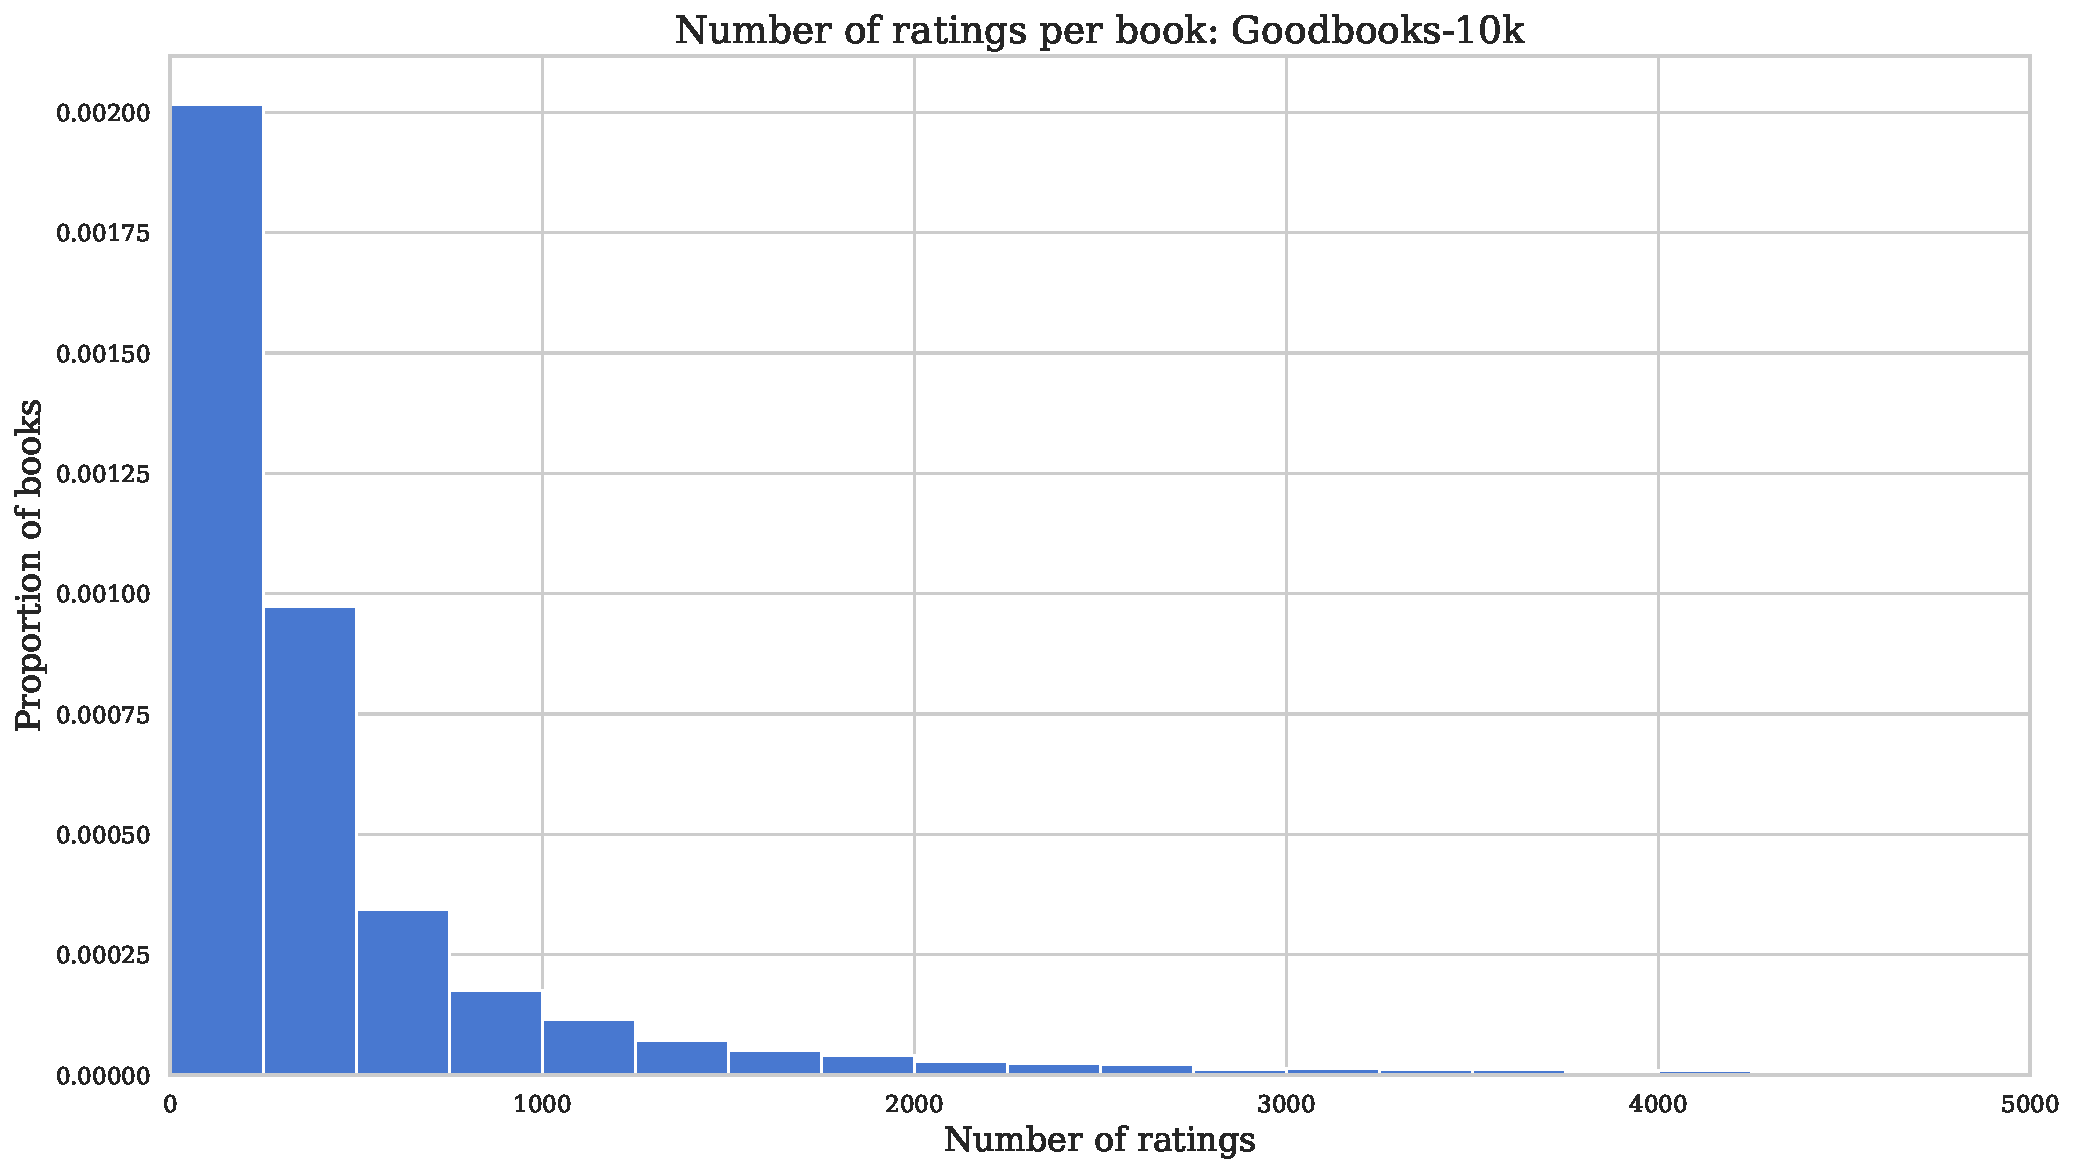
\includegraphics[width=0.75\textwidth]{Figures/3_ratings-distributions/goodbooks-ratings.pdf}
\caption{Goodbooks-10k number of ratings per book.}
\label{fig:goodbooks-items}
\end{figure}

\begin{figure}[H]
\centering
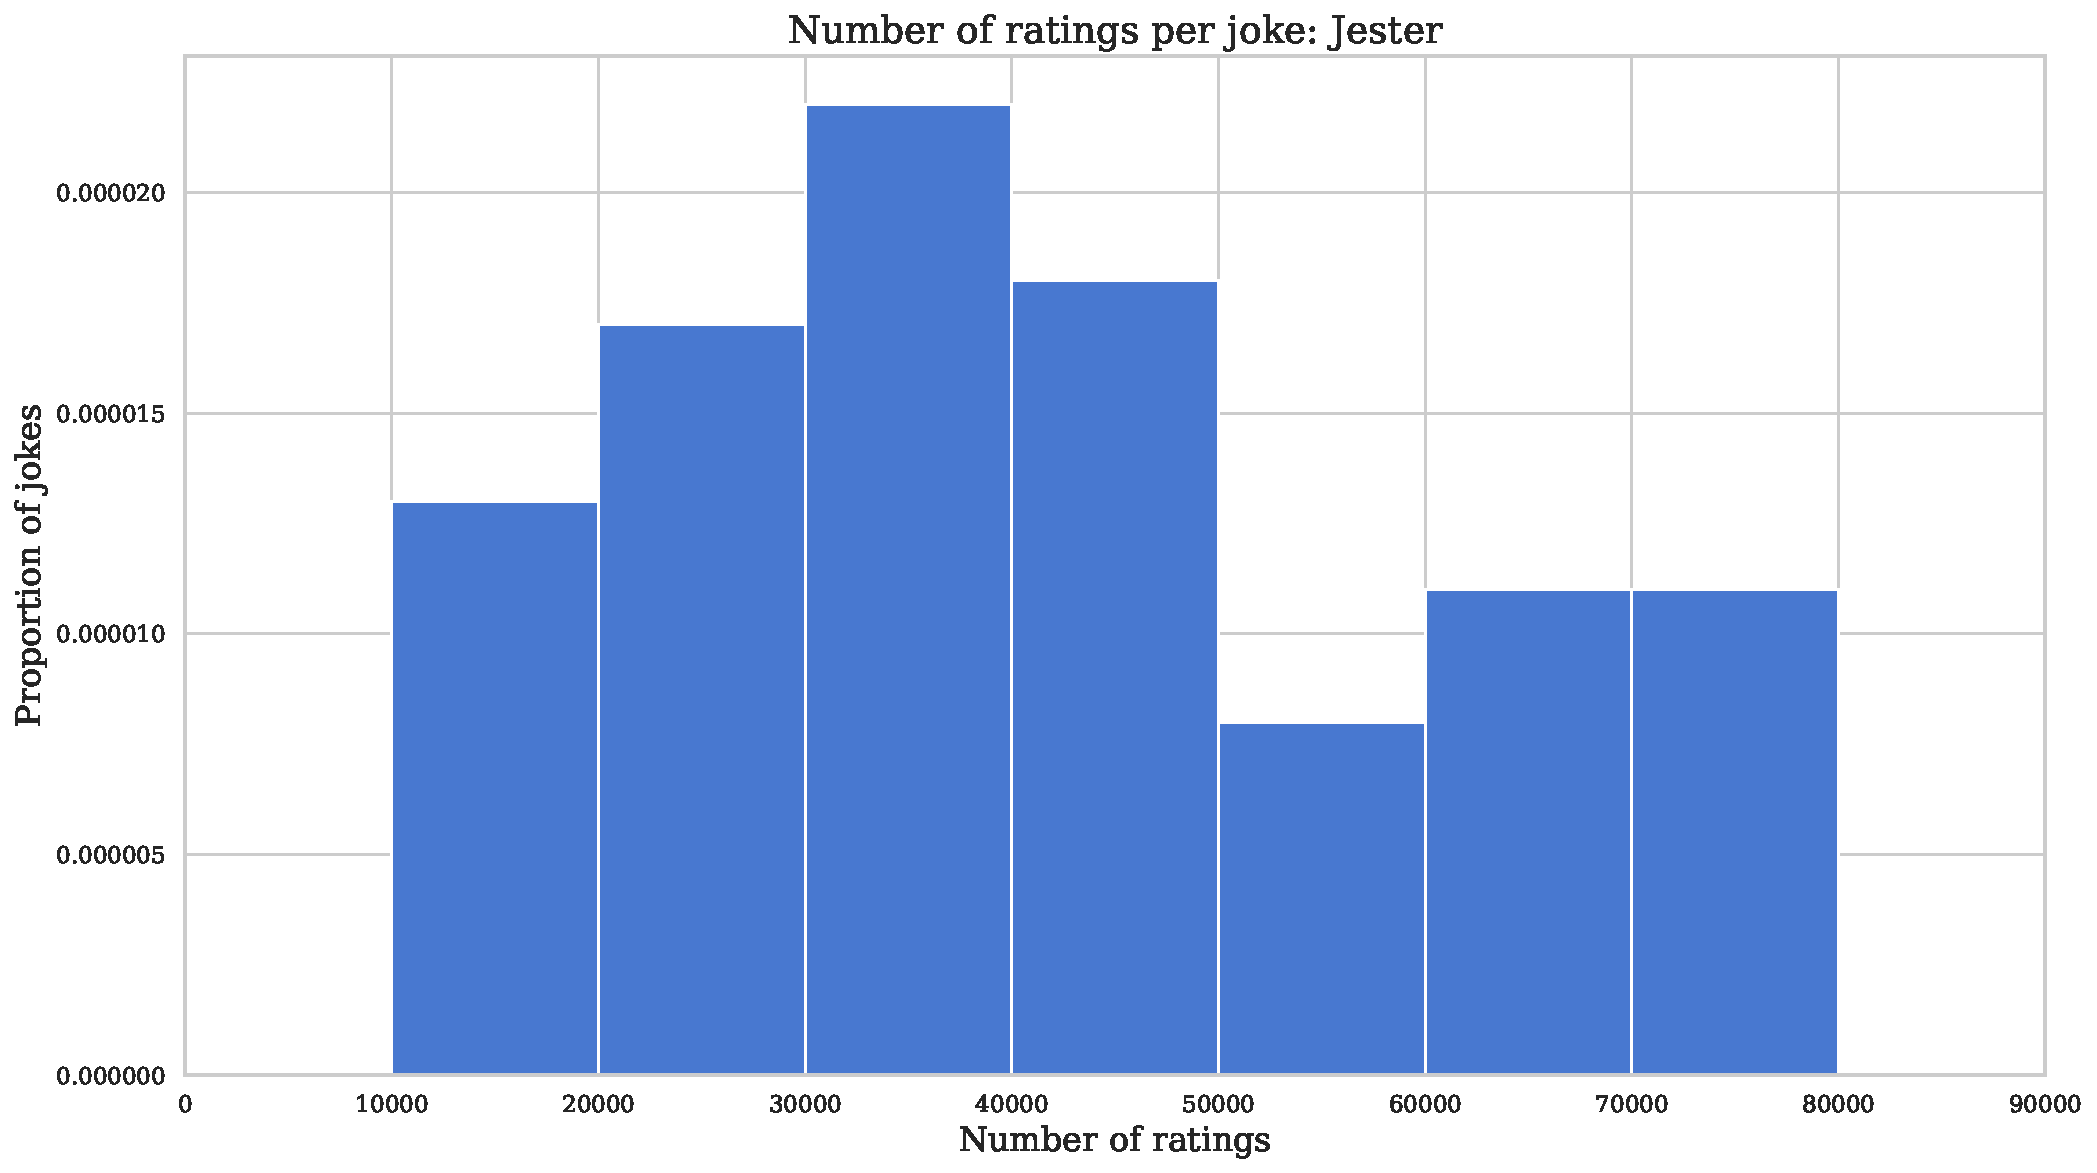
\includegraphics[width=0.75\textwidth]{Figures/3_ratings-distributions/jester_joke-ratings.pdf}
\caption{Jester number of ratings per joke.}
\label{fig:jester-items}
\end{figure}

\subsection{Rating scales}
In all of the datasets, the data are skewed in favour of positive ratings. For example, MovieLens 100k uses a 5-point integer-only rating scale. The middle value of this scale is 3 stars out of 5; however, the mean user rating is 3.53 and the median is 4. In each of the five datasets, both the median and mean values are higher than the middle point of the respective rating scale. Table \ref{tab:ratings-5-number-summaries} shows the 5-number summaries of each dataset.

\begin{table}[H]
\centering
\begin{tabular}{c | c | c | c | c | c | c}
\toprule
\textbf{Name} & \textbf{Min rating} & \textbf{Q2} & \textbf{Median} & \textbf{Q4} & \textbf{Max rating} & \textbf{Mean rating} \\
\midrule
ML 100K & 1 & 3 & 4 & 4 & 5 & 3.53 \\
ML 1M & 1 & 3 & 4 & 4 & 5 & 3.58 \\
ML 10M & 0.5 & 3.0 & 4.0 & 4.0 & 5.0 & 3.51 \\
Goodbooks-10k & 1 & 3 & 4 & 5 & 5 & 3.92 \\
Jester & -10.0 & -3.25 & 1.36 & 5.05 & 10.0 & 0.74 \\
\bottomrule
\end{tabular}
\caption[5-number of summaries of ratings]{Summary of the distribution of ratings in each dataset}
\label{tab:ratings-5-number-summaries}
\end{table}

\section{Distribution of genres}
All MovieLens datasets, as well as Goodbooks-10k, include item metadata. In the case of MovieLens, movies have been tagged with at least one of a total of 18 genres. Books in Goodbooks-10k have been tagged with at least one of 10 genres. Since the items in all four of these datasets may be labelled with one or more genres simultaneously, attempting to predict their genres is considered a multi-label classification problem.

Table \ref{tab:ML-genres} shows the 18 genre categories used in the MovieLens datasets, as well as the proportion of movies that were assigned that genre.

\begin{table}[H]
\centering
\begin{tabular}{c | c | c | c}
\toprule
\textbf{Genre} & \textbf{ML 100k} & \textbf{ML 1M} & \textbf{ML 10M} \\
\midrule
Action & 0.149 & 0.134 & 0.138 \\
Adventure & 0.080 & 0.076 & 0.096 \\
Animation & 0.025 & 0.028 & 0.027 \\
Children's & 0.073 & 0.067 & 0.049 \\
Comedy & 0.300 & 0.314 & 0.350 \\
Crime & 0.065 & 0.054 & 0.105 \\
Documentary & 0.030 & 0.030 & 0.045 \\
Drama & 0.431 & 0.403 & 0.500 \\
Fantasy & 0.013 & 0.018 & 0.051 \\
Film-Noir & 0.014 & 0.012 & 0.014 \\
Horror & 0.054 & 0.091 & 0.095 \\
Musical & 0.033 & 0.030 & 0.041 \\
Mystery & 0.036 & 0.028 & 0.048 \\
Romance & 0.147 & 0.124 & 0.158 \\
Sci-Fi & 0.060 & 0.074 & 0.071 \\
Thriller & 0.149 & 0.131 & 0.160 \\
War & 0.042 & 0.038 & 0.048 \\
Western & 0.016 & 0.018 & 0.026 \\
\bottomrule
\end{tabular}
\caption[Movies per genre as a proportion of the total]{Summary of the distribution of ratings in each dataset}
\label{tab:ML-genres}
\end{table}

From table \ref{tab:ML-genres}, one can see that most of the genres suffer from a significant class imbalance. The drama class is the most balanced, with half of the movies in ML10M being labelled with this genre. The second most well-balanced class is that of comedy, with 35\% of the movies in ML10M being labelled with this genre.